%\documentclass[twocolumn,10pt]{article}
%\usepackage{hyperref}

\documentclass[applications]{gen-bioinformatics}

\makeatletter
\renewcommand\boldmath{\@nomath\boldmath\mathversioo
n{bold}}
\makeatother

\usepackage{amssymb,amsfonts,url,times}
\usepackage{graphics}
\usepackage{amsmath}
\usepackage{dcolumn}
\newcolumntype{.}{D{.}{.}{-1}}
%\usepackage{hlight}

\urlstyle{rm}
\def\email#1{#1}



\newcommand{\Rfunction}[1]{{\texttt{#1}}}
\newcommand{\Robject}[1]{{\texttt{#1}}}
\newcommand{\Rpackage}[1]{{\textit{#1}}}
\newcommand{\Rmethod}[1]{{\texttt{#1}}}
\newcommand{\Rfunarg}[1]{{\texttt{#1}}}
\newcommand{\Rclass}[1]{{\textit{#1}}}
\providecommand{\OO}[1]{\operatorname{O}\left(#1\right)}
 

\author[1]{\pfnm{Shweta}
  \pinit{}
  \psnm{Gopaulakrishnan}}

\author[1]{\pfnm{Samuela}
  \pinit{}
  \psnm{Pollack}}

\author[1]{\pfnm{Benjamin}
  \pinit{}
  \psnm{Stubbs}}

\author[2]{\pfnm{Herv\'e}
  \pinit{}
  \psnm{Pag\`es}}

\author[3]{\pfnm{John}
  \pinit{}
  \psnm{Readey}}

\author[4]{\pfnm{Levi}
  \pinit{}
  \psnm{Waldron}}

\author[5]{\pfnm{Martin}
  \pinit{T}
  \psnm{Morgan}}

\author[1]{\pfnm{Vincent}
  \pinit{J}
  \psnm{Carey}}

\address[1]{\porgdiv{Channing Division of Network Medicine}
  \porgname{Brigham and Women's Hospital}
  \pstreet{181 Longwood Avenue }
  \pcity{Boston}
  \postcode{02115}
  \pcnty{USA}}

\address[2]{\porgdiv{Systems Bioinformatics}
  \porgname{Fred Hutchinson Cancer Research Center}
  \pstreet{Fairview Avenue }
  \pcity{Seattle}
  \postcode{}
  \pcnty{USA}}

\address[3]{
  \porgname{HDF Group}
  \pstreet{}
  \pcity{Seattle}
  \postcode{}
  \pcnty{USA}}

\address[4]{
  \porgname{CUNY}
  \pstreet{}
  \pcity{NY}
  \postcode{}
  \pcnty{USA}}

\address[5]{
  \porgname{RPCI}
  \pstreet{}
  \pcity{Buffalo}
  \postcode{}
  \pcnty{USA}}

 

\begin{document}


\title{restfulSE: a semantically rich interface for cloud-scale genomics}
\maketitle

\begin{abstract}
\begin{subabstract}[Summary]
Bioconductor's \verb+SummarizedExperiment+ class
unites numerical assay quantifications with sample- and
experiment-level metadata.  We describe a deployment
of this data model for data resources that are accessible
via REST APIs.  We illustrate \verb+SummarizedExperiment+s with
HDF Server, HDF Cloud, and Google BigQuery back ends.
\end{subabstract}
\begin{subabstract}[Availability] Package \Rpackage{restfulSE} of Bioconductor
 (\url {www.bioconductor.org}). Open source.
\end{subabstract}
\begin{subabstract}[Contact]reshg@channing.harvard.edu
\end{subabstract}
%\begin{subabstract}[keywords] REST API, HDF5, Bioconductor
\end{abstract}
\section*{Introduction}

The analysis of multiomic archives (like TCGA) and single-cell
transcriptomic experiments (like the 10x 1.3 million mouse neuron
dataset) typically begin with downloads of large files and
conversion of file contents into formats based on local preferences.
In this paper we consider how targeted queries of large remote
genomic data resources can be conducted using methods available
for Bioconductor's \verb+SummarizedExperiment+ class.
This approach can be used to centralize
large data archives and diminish redundant disk
consumption.  Clients for HDF5 or BigQuery data are available in
numerous languages; our Bioconductor interface permits access to
remote archives of genomic data with
familiar and semantically meaningful programmatic idioms.

\section*{Description}

\subsection*{The SummarizedExperiment class and related methods}

Let $X$ denote a matrix of quantifications arising from a genome
scale assay with $G$ assay features measured on $N$ experimental
samples.  In the 10x mouse neuron dataset, $G = 27998$ and $N= 1.3$ million.
When these quantifications are managed in a Bioconductor \verb+SummarizedExperiment X+, the numbers in \verb+X+ are programmatically bound to a $G \times F$
table of feature-level metadata (e.g., gene or transcript names and
characteristics) accessible by the \verb+rowData+ method, and to an $N \times R$ table of sample-level metadata accessible by \verb+colData+ \citep{Huber2015}. 
The idiom \verb+X[G,S]+ expresses filtering of 
the information
to features \verb+G+ and samples \verb+S+.  A \verb+GRanges+ 
instance \citep{Lawrence2013} defining genomic coordinates for features may be bound to \verb+X+,
allowing the use of \verb+subsetByOverlaps+ to isolate features
coincident with or near the elements of a given \verb+GRanges+.
This idea is often used when seeking patterns of variation in
assay elements near regions identified as peaks of factor binding.

\subsection*{Managing quantifications remotely}

\noindent
\textbf{Google BigQuery.} The Institute for Systems Biology Cancer
Genomics Cloud project (ISB-CGC) \citep{ISBCGC} uses 
Google BigQuery to provide access to
various public cancer genomics resources including
The Cancer Genome Atlas (TCGA) and the PanCancer Atlas \citep{Hoadley2018}.
The \verb+pancan_SE+
function of \verb+restfulSE+ constructs queries that derive
SummarizedExperiment instances using quantifications and annotations
for PanCancer atlas experiments
managed in BigQuery tables.  

\noindent
\textbf{HDF Cloud.}  
An AWS S3-based distributed data object model for HDF5
datasets has been implemented by the HDF Group, and
a RESTful API has been defined to structure, populate,
and query HDF5 archives.  Multithreaded queries and
multithreaded query resolution are supported.
The authors have constructed a number of datasets of
interest in genome science for this framework.

\noindent
\textbf{DelayedArray.}
The \verb+restfulSE+ package provides interfaces to 
BigQuery and HDF Cloud so that 
the numerical content lodged in these services
satisfies the Bioconductor \verb+DelayedArray+ API \citep{Pages2018}.  
%Any \verb+DelayedArray+ instance can serve as the \verb+assay+
%component of a \verb+SummarizedExperiment+ instance.  Thus the
%capacities of \verb+SummarizedExperiment+ to bind semantically
%rich metadata to genome-scale assays are extended implicitly to
%data resources for which no standards exist for
%associating substantive metadata.  
In conjunction with the \verb+rhdf5client+ and \verb+bigrquery+ packages,
\verb+restfulSE+ translates filtering and selection operations
which are readily defined using \verb+rowData+, \verb+rowRanges+,
and \verb+colData+ into formal queries resolvable by the HDF5 and
BigQuery services.  Numerical results are transmitted only when needed.

\section*{Results}

\textbf{BigQuery back end.} Figure \ref{pancanPanel} illustrates the 
use of the RESTful SummarizedExperiment protocol
with the ISB-CGC BigQuery back end.  In Figure 5C
of Bailey et al. (2018), it is suggested that
microsatellite instability (MSI) is associated with
different expression signatures of immune cell infiltration
for adenocarcinomas of colon (COAD) and stomach (STAD), and
uterine corpus endometrial carcinoma (UCEC).  Bailey's
detailed quantifications of microsatellite instability
are not available; a categorization of MSI was
obtained from the curatedTCGAData system \citep{Ramos2017}.
Code at the top of Figure \ref{pancanPanel} employs
functions in the BiocOncoTK package that build on
restfulSE functionality to a) authenticate the
user to the BigQuery platform, b) select a tumor
type (COAD) and assay for SummarizedExperiment
construction, c) bind MSI available values as
sample-level data variable \verb+msiTest+, d)
acquire and transform the PD-L1 
(Entrez ID 29126)
expression values, and d) form the stratified boxplot. 
The basic findings of Bailey et al. are replicated.
Enhancement of the code to produce the 3 x 3 tableau
is demonstrated in the BiocOncoTK vignette.

\noindent
\textbf{HDF Cloud back end.}  Figure \ref{hdffig}
demonstrates construction of a RESTful SummarizedExperiment
for expression data on 1.3 million neurons.
The syntax \verb+tenx[g,s]+ generates a delayed selection for
genes \verb+g+ and samples \verb+s+; when the \verb+assay()+
method is invoked, RESTful queries are composed and
shipped to the object store at \verb+URL_hsds()+.
These can be serviced in parallel, with
throughput dependent on the configuration
of the HSDS server and its load at time of request.
Replies can be requested in JSON or binary formats;
rhdf5client utilities handle parsing and modeling the
responses into R matrix structures.

\section*{Performance}

Our considerations of performance focus on reliability,
expressivity, and scalability.  \textit{Reliability:} 
The restfulSE, rhdf5client,
and BiocOncoTK packages are accompanied by detailed unit
tests that compare retrievals to known values.  In the
case of BigQuery table queries, random queries are generated
in BigQuery SQL and in the SummarizedExperiment idiom and
checked for concordance.  \textit{Expressivity:} The code
segments in Figures \ref{pancanPanel} and \ref{hdffig} are
non-trivial but easy to break down.  The joining and
reshaping of pancan-atlas tables in BigQuery corresponding
to the code in Figure \ref{pancanPanel}
can be checked through the query history in the BigQuery
interface.  The acquisition of expression values required
five nested SELECT statements; the query exclusive of
clinical data processing was 6000 characters in length.
The R code is 223 characters including comments.


\begin{figure}[bb]
\begin{verbatim}
library(BiocOncoTK) # uses restfulSE
bq = pancan_BQ() # need CGC_BILLING
seCOAD = bindMSI(buildPancanSE(bq, 
  acronym="COAD", assay="RNASeqv2"))
boxplot(split(log2(as.numeric(assay(
 seCOAD["29126",]))+1), seCOAD$msiTest))
\end{verbatim}
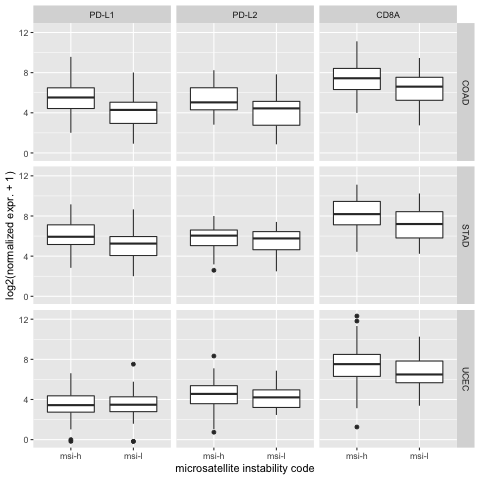
\includegraphics[height=8.0cm]{imm3x3.png}
\caption{Top: Code for base graphics display of boxplot
corresponding to top left panel of lower display.
Bottom: Reassessment of immune infiltrate expression
patterns stratified by microsatellite instability
status and tumor type, as reported in \cite{Bailey2018}.
The vignette for package BiocOncoTK includes all
code needed to produce the nine panel display.}
\label{pancanPanel}
\end{figure}

\begin{figure}[bb]
\begin{verbatim}
eh = ExperimentHub::ExperimentHub()
tenx = eh[["EH554"]]
library(rhdf5client)
tenxA = HSDS_Matrix(URL_hsds(), 
     "/home/reshg/tenx_full.h5") 
assays(tenx) = SimpleList(counts=tenxA)
library(DelayedMatrixStats)
colSums(assay(tenx[,1:4]))
\end{verbatim}
\caption{Code to construct a RESTful SummarizedExperiment
for the 10x Genomics 1.3 million neuron RNA-seq quantifications.
URL\_hsds() returns a string with 
the URL for HDF Kita Lab.  The results are
4046, 2087, 4654, and 3193.}
\label{hdffig}
\end{figure}


\section*{Acknowledgments}
Support for the development of this software was provided by NIH grants
U01 CA214846 (Carey, PI) and U24 CA180996 (Morgan, PI).

\pagebreak

\bibliography{BioC}

\end{document}
